\documentclass[11pt]{article}
\usepackage[margin=1in]{geometry}
\usepackage[T1]{fontenc}
\usepackage[dvipsnames]{xcolor}
\usepackage{amsmath,amsthm,mathtools}
\usepackage{newtxtext,newtxmath}
\usepackage{microtype,bm}
\usepackage{graphicx,booktabs,array}
\usepackage{enumitem}
\usepackage{xurl}
\usepackage[colorlinks=true,linkcolor=MidnightBlue,citecolor=MidnightBlue,urlcolor=MidnightBlue]{hyperref}
\usepackage[nameinlink,noabbrev]{cleveref}
\usepackage{fancyhdr}
\setlength{\headheight}{14pt}
\pagestyle{fancy}
\fancyhf{}
\fancyhead[L]{\small Two-mode extremality for Gaussian quadratic forms}
\fancyhead[R]{\small Research draft}
\fancyfoot[C]{\thepage}
\setlength{\parskip}{3pt}
\setlength{\parindent}{1.2em}
\setlist{itemsep=3pt,topsep=5pt}
\allowdisplaybreaks[2]
\numberwithin{equation}{section}
\newtheorem{theorem}{Theorem}[section]
\newtheorem{proposition}[theorem]{Proposition}
\newtheorem{lemma}[theorem]{Lemma}
\newtheorem{corollary}[theorem]{Corollary}
\theoremstyle{definition}
\newtheorem{definition}[theorem]{Definition}
\newtheorem{example}[theorem]{Example}
\theoremstyle{remark}
\newtheorem{remark}[theorem]{Remark}
\newcommand{\E}{\mathbb E}
\newcommand{\Prob}{\mathbb P}
\newcommand{\R}{\mathbb R}
\newcommand{\N}{\mathbb N}
\newcommand{\Var}{\operatorname{Var}}
\newcommand{\tr}{\operatorname{tr}}
\newcommand{\diag}{\operatorname{diag}}
\newcommand{\supp}{\operatorname{supp}}
\newcommand{\law}{\mathcal L}
\newcommand{\ind}{\mathbf 1}
\newcommand{\Frob}{\mathrm F}
\newcommand{\ds}{\displaystyle}
\newcommand{\dd}{\,\mathrm d}
\newcommand{\eqd}{\overset{\mathrm d}=}
\newcommand{\fourth}{\mathcal F_4}
\newcommand{\gapfour}{\Delta_4}
\DeclareMathOperator{\GammaDist}{Gamma}
\hypersetup{pdftitle={Sharp Two-Mode Extremality for Gaussian Quadratic Fluctuations},pdfauthor={Research manuscript prepared with ChatGPT},pdfsubject={Fixed-skewness sharp moments, spectral stability and tail bounds},pdfkeywords={Gaussian quadratic forms, fourth convex order, skewness, kurtosis, spectral stability}}

\title{\textbf{Sharp Two-Mode Extremality\\for Gaussian Quadratic Fluctuations}\\[6pt]
\large Fixed-skewness moment bounds, spectral rigidity,\\and optimal exponential tail scales}
\author{Research manuscript prepared with ChatGPT}
\date{October 8, 2026}

\begin{document}
\maketitle
\begin{abstract}
Let $Q=\sum_i c_i(g_i^2-1)$, where the $g_i$ are independent standard Gaussian variables, $\sum_i c_i^2=1$, and $\delta=\sum_i c_i^3$. We prove that the same two-coordinate quadratic form maximizes $\E f(Q)$, at every fixed $\delta$, for every twice continuously differentiable $f$ with convex second derivative and polynomial growth. The maximizer is
\[
Y_\delta=a(g^2-1)-b(h^2-1),\qquad
 a,b\geq0,\quad a^2+b^2=1,\quad a^3-b^3=\delta.
\]
Consequently, the absolute-moment extremal problem at fixed variance and skewness is solved for every real order $p\geq3$, including all equality cases. The key is the sharp coefficient enclosure $-b\leq c_i\leq a$; its convex-chord weights are exactly $b^2$ and $a^2$, so the envelope is an attainable quadratic form rather than an auxiliary law. We obtain the exact skewness--kurtosis frontier, explicit moment-deficit and spectral-distance inequalities, and a sharp exponential-moment envelope with a closed-form Chernoff optimizer. At zero skewness, the extremizer is a product of two independent Gaussians; the fourth-moment upper bound improves from $60$ to $36$ under our variance-two normalization. The squared spectral-distance constant $4$ at zero skewness is optimal. We also treat common-shape Gamma inputs and centered infinitely divisible inputs, and provide exact-arithmetic checks and reproducible numerical diagnostics.

\smallskip
\noindent\textbf{Status.} This is an unrefereed research manuscript with self-contained proofs and computational checks, not a Lean-certified result. The fixed-skewness strengthening is proposed as a contribution relative to the primary sources examined; bibliographic priority has not been independently established.
\end{abstract}
\vspace{4pt}
\noindent\textbf{Keywords:} Gaussian quadratic form; fourth convex order; skewness; sharp moments; spectral stability; Gamma distribution.\\
\textbf{Mathematics Subject Classification:} 60E15, 60E07, 60G15; 15A42.
\newpage
\begingroup
\small
\setlength{\parskip}{0pt}
\setlength{\baselineskip}{11pt}
\tableofcontents
\endgroup
\newpage

\section{The problem and the strengthening}
\label{sec:intro}

For $G\sim N(0,I_n)$, a centered quadratic observable has the spectral representation
\begin{equation}\label{eq:matrix-model}
G^{\mathsf T}MG-\tr M\eqd\sum_{i=1}^n\lambda_i(g_i^2-1),
\end{equation}
where $M$ is real symmetric. This covers quadratic energy fluctuations and Gaussian estimates of matrix traces. Its distribution depends on the full spectrum, but applications often retain only a few trace statistics. The question here is exact: \emph{what is the largest possible absolute moment when the second and third traces are fixed?}

The general moment-extremal question is posed by Bartczak, Nayar, and Zwara \cite{BNZ2021}. Pang \cite{Pang2026} proves rank-one extremality for all real $p\geq4$ without fixing skewness, and obtains a skewness-dependent Gamma envelope for a larger class of test functions. Our result sharpens that envelope inside each fixed-skewness class: the comparison variable is an actual rank-two quadratic form, and therefore gives the exact conditional optimum, not merely an upper estimate. We do not claim to settle the remaining unconditioned problem throughout $2<p<4$.

The source of inspiration requested for this project is the OpenAI mathematics repository \cite{OpenAIRepository}. Its orthogonally invariant Ising family includes explicit Gaussian quadratic-form mean and variance calculations \cite{OpenAIGaussian}. We use that elementary spectral-fluctuation perspective, not the family's all-temperature spin-glass assertion. No unverified major theorem from that repository is a premise of any proof below.

\subsection{Normalization and the class of observables}
For $M\ne0$, put
\begin{equation}\label{eq:normalization}
s=\|M\|_{\Frob}=\sqrt{\tr(M^2)},\qquad
c_i=\lambda_i/s,\qquad
Q=\frac{G^{\mathsf T}MG-\tr M}{s},\qquad
\delta=\frac{\tr(M^3)}{\tr(M^2)^{3/2}}.
\end{equation}
Then $\sum_i c_i^2=1$, $\delta=\sum_i c_i^3\in[-1,1]$, and
\begin{equation}\label{eq:first-three}
\E Q=0,\qquad \E Q^2=2,\qquad \E Q^3=8\delta.
\end{equation}
The standardized skewness is $\gamma=2\sqrt2\,\delta$. Zero skewness means $\tr(M^3)=0$, \emph{not} $\tr M=0$; it does not imply a spectrum symmetric about zero.

\begin{definition}\label{def:F4}
Let $\fourth$ be the class of functions $f\in C^2(\R)$ such that $f''$ is convex and, for some $C,m<\infty$,
\[
|f(x)|+|f'(x)|+|f''(x)|\leq C(1+|x|^m),\qquad x\in\R.
\]
Write $X\preceq_4 Y$ if $\E f(X)\leq\E f(Y)$ for every $f\in\fourth$.
\end{definition}
This is a polynomial-growth version of generalized fourth convex order; see \cite{Denuit1998}. Polynomials of degree at most three, with either sign, belong to $\fourth$, so an ordering requires matching the first three moments. For every real $p\geq3$, $f(x)=|x|^p$ is in $\fourth$.

\subsection{What is and is not claimed}
The main contribution is a sharp, dimension-independent extremal theorem at prescribed $\delta$, with an attained optimizer and quantitative rigidity. The improvement is not an asymptotic expansion and not restricted to integer moments, positive semidefinite matrices, or symmetric coefficient lists. General tail inequalities such as Hanson--Wright and chaos moment estimates \cite{HansonWright1971,RudelsonVershynin2013,Latala2006} address different, non-exact objectives.

The proof adapts the convex-chord and compound-Poisson comparison mechanism in \cite{Pang2026}, in the broader setting of comparison by L\'evy measures \cite{Bergenthum2007}. The new ingredient is an asymmetric enclosure forced jointly by the second and third coefficient sums. This enclosure makes the endpoint law feasible in the original spectral optimization problem.

The manuscript does not assert pointwise tail domination by its extremizer, optimal Chernoff prefactors, or improved algorithms for arbitrary non-Gaussian inputs. All comparisons are proved under explicitly stated hypotheses.

\section{The attained extremal law}
\label{sec:main}

For $\delta\in[-1,1]$, define $a=a(\delta)$ and $b=b(\delta)$ by
\begin{equation}\label{eq:ab}
a,b\geq0,\qquad a^2+b^2=1,\qquad a^3-b^3=\delta.
\end{equation}
These equations have a unique solution. A convenient explicit parameterization is
\begin{equation}\label{eq:trig}
\eta=2\sin\!\left(\frac{\arcsin\delta}{3}\right),\qquad
S=\sqrt{2-\eta^2},\qquad
 a=\frac{S+\eta}{2},\qquad b=\frac{S-\eta}{2}.
\end{equation}
Thus $S=a+b$, $\eta=a-b$, $ab=(1-\eta^2)/2$, and
$\delta=(3\eta-\eta^3)/2$. In particular $a(0)=b(0)=2^{-1/2}$, while $(a(1),b(1))=(1,0)$.

Let $g,h$ be independent standard normal variables and set
\begin{equation}\label{eq:Y}
Y_\delta=a(g^2-1)-b(h^2-1).
\end{equation}
Both $Q$ and $Y_\delta$ have the moments in \eqref{eq:first-three}.

\begin{theorem}[Sharp fixed-skewness comparison]\label{thm:main}
Let $g_1,\ldots,g_n$ be independent standard normal variables. Let $c_1,\ldots,c_n\in\R$ satisfy $\sum_i c_i^2=1$, and let
$Q=\sum_i c_i(g_i^2-1)$ and $\delta=\sum_i c_i^3$. Then
\begin{equation}\label{eq:order}
Q\preceq_4 Y_\delta.
\end{equation}
For every real $p\geq3$,
\begin{equation}\label{eq:moments-main}
\E|Q|^p\leq F_p(\delta):=\E|Y_\delta|^p.
\end{equation}
Equality in \eqref{eq:moments-main}, for any one such $p$, holds if and only if the nonzero coefficients, counting multiplicity, are $a$ and $-b$, with a zero endpoint omitted. Thus the same feasible spectrum solves every one of these fixed-skewness maximization problems.
\end{theorem}

For $|\delta|<1$, this is a rank-two maximizer with one positive and one negative eigenvalue. For $\delta=\pm1$, the only feasible spectra are the corresponding rank-one spectra. If a fixed ambient dimension is required, the interior assertion is understood for $n\geq2$; every $\delta\in[-1,1]$ is then feasible.

\begin{corollary}[Matrix form]\label{cor:matrix}
Under \eqref{eq:normalization}, for $p\geq3$,
\[
\|G^{\mathsf T}MG-\tr M\|_p
\leq \|M\|_{\Frob}\,F_p(\delta)^{1/p}.
\]
Equality holds precisely when the normalized nonzero eigenvalues of $M$ are $a$ and $-b$, omitting a zero endpoint.
\end{corollary}

An elementary two-dimensional integral evaluates the exact constant:
\begin{equation}\label{eq:F-integral}
F_p(\delta)=\frac1{2\pi}\int_{\R^2}
\left|a(x^2-1)-b(y^2-1)\right|^p e^{-(x^2+y^2)/2}\dd x\dd y.
\end{equation}
The symmetry $F_p(-\delta)=F_p(\delta)$ follows by interchanging $g$ and $h$. Computing \eqref{eq:F-integral} numerically is separate from proving its extremal property.

\section{Sharp coefficient geometry}
\label{sec:geometry}

\begin{lemma}[Optimal asymmetric enclosure]\label{lem:enclosure}
Under the hypotheses of \cref{thm:main}, every coefficient belongs to $[-b,a]$.
\end{lemma}
\begin{proof}
For a real vector $z$, the elementary norm inequality gives
\[
\left|\sum_j z_j^3\right|\leq \sum_j|z_j|^3
\leq\left(\sum_j z_j^2\right)^{3/2}.
\]
If $c_i=t\geq0$, apply this to the remaining coordinates:
\[
\delta\geq t^3-(1-t^2)^{3/2}.
\]
The function $H(t)=t^3-(1-t^2)^{3/2}$ is strictly increasing on $[0,1]$, and $H(a)=\delta$. Hence $t\leq a$. If $c_i=-t\leq0$, the opposite inequality on the remaining coordinates gives
$\delta\leq(1-t^2)^{3/2}-t^3$, and therefore $t\leq b$. The spectrum $(a,-b)$ attains both endpoints, so the enclosure cannot be improved from these constraints alone.
\end{proof}

\begin{lemma}[The feasible endpoint chord]\label{lem:chord}
For every convex $\phi:[-b,a]\to\R$,
\begin{equation}\label{eq:chord}
\sum_i c_i^2\phi(c_i)\leq a^2\phi(a)+b^2\phi(-b).
\end{equation}
\end{lemma}
\begin{proof}
The measure $\mu=\sum_i c_i^2\delta_{c_i}$ is a probability measure with mean $\delta$. For $z\in[-b,a]$,
\[
\phi(z)\leq\frac{z+b}{S}\phi(a)+\frac{a-z}{S}\phi(-b).
\]
Integrating and using
\begin{equation}\label{eq:weights}
\frac{\delta+b}{S}=a^2,\qquad
\frac{a-\delta}{S}=b^2
\end{equation}
proves the assertion. For example, $\delta+b=a^3-b^3+b=a^3+a^2b=a^2S$.
\end{proof}

The identities \eqref{eq:weights} are decisive. Using only the coarser interval $[-1,1]$ gives endpoint masses $(1+\delta)/2$ and $(1-\delta)/2$, which lead to an auxiliary Gamma law. The sharp interval instead produces exactly the squared coefficients of the two-coordinate feasible spectrum.

\begin{lemma}[An exact polynomial defect]\label{lem:defect}
Put
\begin{equation}\label{eq:defect}
T_\delta=a^4+b^4,\qquad
\gapfour=T_\delta-\sum_i c_i^4.
\end{equation}
Then
\begin{equation}\label{eq:defect-factor}
\gapfour=\sum_i c_i^2(a-c_i)(c_i+b)\geq0.
\end{equation}
\end{lemma}
\begin{proof}
Expand the right side and use the second and third coefficient sums:
\[
\sum_i c_i^2(a-c_i)(c_i+b)
=ab+(a-b)\delta-\sum_i c_i^4.
\]
The identity $ab+(a-b)(a^3-b^3)=a^4+b^4$ follows from $a^2+b^2=1$. Nonnegativity follows from \cref{lem:enclosure}.
\end{proof}

\section{A self-contained interpolation proof}
\label{sec:proof}

\subsection{The centered chi-square L\'evy representation}
For $Z=g^2-1$ and $t<1/2$,
\begin{equation}\label{eq:psi}
\psi(t):=\log\E e^{tZ}=-t-\tfrac12\log(1-2t)
=\int_0^\infty(e^{tr}-1-tr)\,\frac{e^{-r/2}}{2r}\dd r.
\end{equation}
One can verify the last equality by differentiating in $t$, obtaining $(1-2t)^{-1}-1$, and evaluating both sides at $t=0$.
Write
\[
\nu(\dd r)=\frac{e^{-r/2}}{2r}\dd r,\qquad r>0.
\]
The measure has infinite total mass but finite second moment. If $R$ has Gamma shape $2$ and scale $2$, with density $r e^{-r/2}/4$, then
\begin{equation}\label{eq:R-representation}
\int q(r)\nu(\dd r)=2\E\frac{q(R)}{R^2},
\end{equation}
whenever the integrals are defined. The scale convention is used throughout this manuscript.

\subsection{Finite jump measures and their derivative}
For $\varepsilon>0$, truncate at $r>\varepsilon$ and define finite measures on $\R$ by
\begin{align}
\int q(y)\nu_{0,\varepsilon}(\dd y)
&=\sum_{i:c_i\ne0}\int_\varepsilon^\infty q(c_ir)\nu(\dd r),\label{eq:nu0}\\
\int q(y)\nu_{1,\varepsilon}(\dd y)
&=\int_\varepsilon^\infty
\bigl[\ind_{a>0}q(ar)+\ind_{b>0}q(-br)\bigr]\nu(\dd r).\label{eq:nu1}
\end{align}
Set $\nu_{u,\varepsilon}=(1-u)\nu_{0,\varepsilon}+u\nu_{1,\varepsilon}$, $0\leq u\leq1$. Let $X_{u,\varepsilon}$ be the centered compound-Poisson variable with this jump measure:
\[
X_{u,\varepsilon}=\sum_{j=1}^{N}J_j-\int y\nu_{u,\varepsilon}(\dd y),
\]
where $N$ has mean $\nu_{u,\varepsilon}(\R)$ and the jumps have its normalized law.

For a bounded $C^1$ test function $q$ with bounded derivative, differentiating the absolutely convergent Poisson series gives
\begin{align}\label{eq:poisson-derivative}
\frac{\mathrm d}{\mathrm du}\E q(X_{u,\varepsilon})
=\int \E\bigl[q(X_{u,\varepsilon}+y)-q(X_{u,\varepsilon})
-yq'(X_{u,\varepsilon})\bigr]
(\nu_{1,\varepsilon}-\nu_{0,\varepsilon})(\dd y).
\end{align}
For completeness, differentiation of the intensity produces the add-one-jump difference $q(X+y)-q(X)$. Differentiation of the deterministic centering produces $-yq'(X)$. The signed measure has finite total variation and finite first moment, so both differentiated terms are integrable. At $u=0,1$ use one-sided derivatives. This also follows from the standard finite-measure perturbation formula, but no such external theorem is needed here.

For twice continuously differentiable test functions, Taylor's identity
\begin{equation}\label{eq:Taylor}
q(x+y)-q(x)-yq'(x)
=y^2\int_0^1(1-v)q''(x+vy)\dd v
\end{equation}
then transforms the derivative into
\begin{align}\label{eq:derivative-chord}
\frac{\mathrm d}{\mathrm du}\E q(X_{u,\varepsilon})
=2\E\Biggl[\ind_{R>\varepsilon}\int_0^1(1-v)
\Bigl\{&a^2q''(X_{u,\varepsilon}+vaR)
+b^2q''(X_{u,\varepsilon}-vbR)\notag\\
&-\sum_i c_i^2q''(X_{u,\varepsilon}+vc_iR)\Bigr\}\dd v\Biggr],
\end{align}
where $R$ is independent of $X_{u,\varepsilon}$.

\subsection{Growth bounds and removal of truncation}
We give the integrability details because they will also justify a quantitative deficit identity. For $|t|<1/2$ and $|z|\leq1$, the series of \eqref{eq:psi} gives
\begin{equation}\label{eq:psi-bound}
0\leq\psi(tz)
\leq\frac{t^2z^2}{1-2|t|}.
\end{equation}
Indeed, the absolute coefficient of $(tz)^k$ is $2^{k-1}/k\leq2^{k-2}$ for $k\geq2$. Since $e^{ty}-1-ty\geq0$ for real $ty$, truncation decreases the real cumulant exponent. Both endpoint spectra have squared sum one, so
\begin{equation}\label{eq:uniform-exp}
\sup_{u\in[0,1],\,\varepsilon>0}
\E e^{|X_{u,\varepsilon}|/4}\leq2e^{1/8}.
\end{equation}
In particular, polynomial moments of every order are uniformly integrable.

For $f\in\fourth$, multiply $f$ by a smooth cutoff equal to one on $[-N,N]$ and zero outside $[-2N,2N]$. The resulting $f_N$ and its first two derivatives satisfy polynomial bounds uniform in $N$. Although $f_N''$ need not be convex, the identity \eqref{eq:derivative-chord}, integrated over $u$, applies to $f_N$. Letting $N\to\infty$ is valid by \eqref{eq:uniform-exp}, the polynomial growth bounds, and the finite moments of $R$. After taking this limit, convexity of $f''$ and \cref{lem:chord} show that the integrand is nonnegative. Hence
\[
\E f(X_{0,\varepsilon})\leq\E f(X_{1,\varepsilon}).
\]

The characteristic exponents of $X_{u,\varepsilon}$ converge as $\varepsilon\downarrow0$ to those with untruncated jump measures. The limit $X_u$ can be written explicitly as
\begin{equation}\label{eq:interpolant}
X_u=\sum_i c_i\bigl(A_{i,u}-(1-u)\bigr)
+a(B_u-u)-b(C_u-u),
\end{equation}
where all variables are independent and
\[
A_{i,u}\sim\GammaDist\!\left(\frac{1-u}{2},2\right),\qquad
B_u,C_u\sim\GammaDist\!\left(\frac u2,2\right).
\]
A Gamma variable of shape zero is zero. Thus $X_0\eqd Q$, $X_1\eqd Y_\delta$, and, for every $u$,
\begin{equation}\label{eq:interpolant-moments}
\E X_u=0,\qquad \Var X_u=2,\qquad \E X_u^3=8\delta.
\end{equation}
Weak convergence together with \eqref{eq:uniform-exp} permits passage to expectations of polynomial-growth functions. This proves \eqref{eq:order}.

\subsection{An exact deficit identity}
The same limiting argument applied to the integrated identity gives more than an inequality. Define
\begin{equation}\label{eq:chord-gap-definition}
\mathcal D_f(x,r,v)=a^2f''(x+var)+b^2f''(x-vbr)
-\sum_i c_i^2f''(x+vc_ir).
\end{equation}
Then
\begin{equation}\label{eq:deficit-identity}
\boxed{\quad
\E f(Y_\delta)-\E f(Q)
=2\int_0^1\int_0^1(1-v)\,
\E\mathcal D_f(X_u,R,v)\dd v\dd u.
\quad}
\end{equation}
For the passage to the limit, each summand is bounded in absolute value by a constant times $1+|X_{u,\varepsilon}|^m+R^m$. Higher uniform moments give uniform integrability for the product laws, and then dominated convergence in $u,v$ applies. This proves \eqref{eq:deficit-identity} without assuming a fourth classical derivative.

\subsection{Equality cases, including the endpoint $p=3$}
For $p>3$, the function
$f''(x)=p(p-1)|x|^{p-2}$ is strictly convex. If any nonzero $c_i$ lies strictly between $-b$ and $a$, the corresponding chord inequality is strict for every $v>0$, $R>0$. Thus \eqref{eq:deficit-identity} gives a strictly positive moment deficit.

For $p=3$, $f''(x)=6|x|$ is only piecewise linear. Suppose $a,b>0$. At every $0<u<1$, the independent difference $aB_u-bC_u$ has support equal to $\R$ and assigns positive probability to every nonempty open interval. Convolving with the remaining summands preserves this property. Conditional on $v,R>0$, the event
\[
-vaR<X_u<vbR
\]
has positive probability. On this event the two chord endpoints straddle zero, and the chord for absolute value is strictly above its graph at every interior point. Therefore a nonzero interior coefficient again forces a strictly positive deficit.

If no such coefficient exists, all nonzero coefficients are endpoints. Their total squared masses are $a^2$ and $b^2$ by \eqref{eq:weights}. Since each occurrence of $a$ already has mass $a^2$, and likewise for $-b$, there is exactly one occurrence of each nonzero endpoint. At $\delta=\pm1$, equality in the elementary $\ell_3$--$\ell_2$ bound already forces the corresponding rank-one spectrum. This completes the proof of \cref{thm:main}.

\section{The exact skewness--kurtosis frontier}
\label{sec:kurtosis}

The cumulants of $Q$ are
\begin{equation}\label{eq:cumulants}
\kappa_1(Q)=0,\qquad
\kappa_r(Q)=2^{r-1}(r-1)!\sum_i c_i^r\quad(r\geq2).
\end{equation}
In particular,
\begin{equation}\label{eq:fourth-sixth}
\E Q^4=12+48\sum_i c_i^4,
\end{equation}
and
\begin{equation}\label{eq:sixth}
\E Q^6=120+1440\sum_i c_i^4+640\delta^2+3840\sum_i c_i^6.
\end{equation}
These identities follow either by expanding \eqref{eq:psi} or by the recurrence in \cref{app:moments}.

\begin{theorem}[Sharp kurtosis at prescribed skewness]\label{thm:kurtosis}
With $\eta$ as in \eqref{eq:trig}, every normalized Gaussian quadratic form satisfies
\begin{equation}\label{eq:kurtosis-frontier}
\frac{\E Q^4}{(\E Q^2)^2}
\leq 3+12T_\delta
=15-6(1-\eta^2)^2.
\end{equation}
Every point on this upper frontier is attained by $Y_\delta$, and equality characterizes its spectrum. Moreover,
\begin{equation}\label{eq:fourth-exact-deficit}
\E Y_\delta^4-\E Q^4=48\gapfour.
\end{equation}
\end{theorem}
\begin{proof}
Apply \cref{lem:defect} to \eqref{eq:fourth-sixth}. Finally,
$T_\delta=(a^2+b^2)^2-2a^2b^2=1-(1-\eta^2)^2/2$. Equality in \eqref{eq:defect-factor} forces all nonzero coefficients to be endpoints, as above.
\end{proof}

The upper standardized kurtosis is $9$ at zero skewness and $15$ at maximal skewness magnitude $2\sqrt2$. For small skewness,
\begin{equation}\label{eq:kurtosis-expansion}
3+12T_\delta
=9+\frac{16}{3}\delta^2+\frac{32}{81}\delta^4+O(\delta^6)
=9+\frac23\gamma^2+\frac1{162}\gamma^4+O(\gamma^6).
\end{equation}
The expansion describes the curvature of an exact attainable boundary, not merely a bound on its leading terms.

\begin{figure}[htbp]
\centering
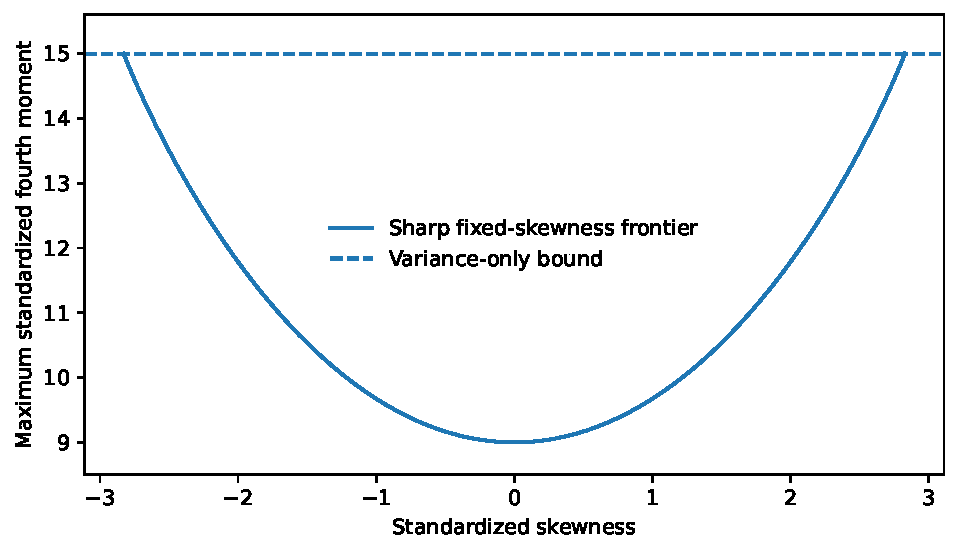
\includegraphics[width=.79\textwidth]{figures/kurtosis_frontier.pdf}
\caption{The exact upper standardized kurtosis as a function of standardized skewness $\gamma=2\sqrt2\delta$. The horizontal reference is the variance-only upper bound. Both axes concern the entire class of real symmetric Gaussian quadratic forms.}
\label{fig:kurtosis}
\end{figure}

\subsection{Zero skewness: all absolute moments in closed form}
At $\delta=0$,
\[
Y_0=\frac{g^2-h^2}{\sqrt2}\eqd\sqrt2\,UV,
\]
where $U=(g+h)/\sqrt2$ and $V=(g-h)/\sqrt2$ are independent standard normal variables. Thus
\begin{corollary}[Sharp zero-skewness constants]\label{cor:zero}
If $\sum_i c_i^2=1$ and $\sum_i c_i^3=0$, then, for every $p\geq3$,
\begin{equation}\label{eq:zero-moment}
\E|Q|^p\leq
\frac{2^{3p/2}}{\pi}\Gamma\!\left(\frac{p+1}{2}\right)^2.
\end{equation}
Equality holds precisely for $(2^{-1/2},-2^{-1/2})$, with zero coefficients appended. For integers $k\geq2$, the right side at $p=2k$ is $2^k[(2k-1)!!]^2$.
\end{corollary}
\begin{proof}
Use \cref{thm:main}, independence of $U,V$, and
$\E|U|^p=2^{p/2}\Gamma((p+1)/2)/\sqrt\pi$.
\end{proof}

\begin{table}[htbp]
\centering
\caption{Attained moment maxima under variance $2$ and zero skewness.}
\begin{tabular}{@{}ccc@{}}
\toprule
Order $p$ & $\sup\E|Q|^p$ & Attaining law\\
\midrule
$3$ & $16\sqrt2/\pi\approx7.202530529$ & $\sqrt2 UV$\\
$4$ & $36$ & $\sqrt2 UV$\\
$6$ & $1800$ & $\sqrt2 UV$\\
$8$ & $176400$ & $\sqrt2 UV$\\
\bottomrule
\end{tabular}
\label{tab:moments}
\end{table}

For comparison, the universal variance-only fourth-moment maximum is $60$, attained by $g^2-1$. Pang's auxiliary variable at skewness $\delta$ has Gamma shapes $(1+\delta)/4$ and $(1-\delta)/4$, scale $2$, and fourth moment $60$ for every $\delta$ \cite{Pang2026}. Its comparison therefore loses exactly the feature captured by \eqref{eq:kurtosis-frontier}. Indeed, applying that earlier envelope to the feasible $Y_\delta$ places our attained bound below it for every admissible test function.

\begin{example}[Zero skewness without a symmetric spectrum]\label{ex:nonsymmetric}
The normalized spectrum
\[
(c_1,c_2,c_3,c_4)=\frac{(3,4,5,-6)}{\sqrt{86}}
\]
has cubic sum zero because $27+64+125=216$. It is not symmetric, and its fifth coefficient sum is $-3384/86^{5/2}\ne0$, so the corresponding law is not symmetric either. Nevertheless, \eqref{eq:zero-moment} applies. Its fourth moment is
\[
12+48\frac{2258}{7396}\approx26.654407788<36.
\]
\end{example}

\section{Quantitative moment deficits}
\label{sec:moment-stability}

The enclosure and the exact defect identity make the comparison quantitative. Let
\begin{equation}\label{eq:rho}
\rho=\Prob(1\leq R\leq2)=\frac32e^{-1/2}-2e^{-1}>0.
\end{equation}

\begin{theorem}[Explicit moment stability]\label{thm:moment-stability}
Under \cref{thm:main}, for $p\geq4$,
\begin{equation}\label{eq:moment-stability-large}
F_p(\delta)-\E|Q|^p\geq
4\Gamma(p)S^{p-4}\gapfour.
\end{equation}
For $3<p<4$,
\begin{equation}\label{eq:moment-stability-small}
F_p(\delta)-\E|Q|^p\geq C_p\gapfour,
\qquad
C_p=\frac{p(p-1)(p-2)(p-3)}{24}\,4^{p-4}\rho.
\end{equation}
At $p=4$, the exact coefficient is $48$, by \eqref{eq:fourth-exact-deficit}, rather than the weaker $24$ supplied by \eqref{eq:moment-stability-large}.
\end{theorem}

\begin{proof}
For $q=p-2$ and $w_i=(c_i+b)/S$, the inner chord gap in \eqref{eq:deficit-identity}, divided by $p(p-1)$, is a weighted sum of
\[
H_q(w;x_+,x_-)
=w|x_+|^q+(1-w)|x_-|^q
-|wx_++(1-w)x_-|^q,
\]
with $x_+=X_u+vaR$, $x_-=X_u-vbR$, and weights $c_i^2$. We have
\begin{equation}\label{eq:w-defect}
\sum_i c_i^2w_i(1-w_i)=\frac{\gapfour}{S^2}.
\end{equation}

Suppose $q\geq2$. The scalar Clarkson inequality gives
\[
H_q(1/2;x_+,x_-)\geq2^{-q}|x_+-x_-|^q.
\]
As a function of $w$, $H_q$ is concave and vanishes at $0,1$. Comparing with the chords on $[0,1/2]$ and $[1/2,1]$ yields
\begin{equation}\label{eq:power-gap}
H_q(w;x_+,x_-)
\geq2^{1-q}w(1-w)|x_+-x_-|^q.
\end{equation}
Since $x_+-x_-=vRS$, substitution into \eqref{eq:deficit-identity} gives
\begin{align*}
F_p(\delta)-\E|Q|^p
&\geq2p(p-1)2^{1-q}S^{q-2}\gapfour\,
\E R^q\int_0^1(1-v)v^q\dd v\\
&=4\Gamma(p)S^{p-4}\gapfour,
\end{align*}
because $\E R^q=2^q\Gamma(q+2)$ and
$\int_0^1(1-v)v^q\dd v=1/[(q+1)(q+2)]$.

Now suppose $1<q<2$. On $[-4,4]$, the function $|x|^q$ is strongly convex with modulus
$\mu_q=q(q-1)4^{q-2}$. This follows by subtracting $\mu_q x^2/2$: its derivative is nondecreasing, including across zero. Therefore, for $x_+,x_-\in[-4,4]$,
\[
H_q(w;x_+,x_-)\geq\frac{\mu_q}{2}w(1-w)(x_+-x_-)^2.
\]
Restrict \eqref{eq:deficit-identity} to $|X_u|\leq2$ and $1\leq R\leq2$. On this event both endpoints lie in $[-4,4]$. By \eqref{eq:interpolant-moments} and Chebyshev's inequality,
$\Prob(|X_u|\leq2)\geq1/2$, uniformly in $u$. Independence, \eqref{eq:w-defect}, $R^2\geq1$ on the restricted event, and
$\int_0^1(1-v)v^2\dd v=1/12$ now give
\[
F_p(\delta)-\E|Q|^p
\geq\frac{p(p-1)\mu_q\rho}{24}\gapfour,
\]
which is \eqref{eq:moment-stability-small}.
\end{proof}

The constants above are explicit but, except for the exact fourth-moment identity, are not claimed optimal. The $p=3$ equality theorem remains valid; the argument here does not provide a positive quantitative constant at that endpoint.

\section{Spectral rigidity and its optimal zero-skewness constant}
\label{sec:rigidity}

Let $\mathcal O_\delta$ consist of the spectra $(a,-b,0,\ldots)$ under coordinate permutations. To compare vectors of arbitrary dimensions, append zero coordinates as necessary. Define
\begin{equation}\label{eq:distance}
D(c,\mathcal O_\delta)^2
=\inf_{z\in\mathcal O_\delta}\sum_i(c_i-z_i)^2.
\end{equation}
Appending zeros is material for one-sign spectra: it allows the missing signed mode to occupy a new coordinate. When $c$ has both signs, no extension of the ambient space is needed. For matrices, this is the distance between eigenvalue lists, equivalently the minimum Frobenius distance to the orthogonal orbit after the same zero extension.

\begin{theorem}[Spectral rigidity]\label{thm:rigidity}
If $|\delta|<1$, then
\begin{equation}\label{eq:rigidity}
D(c,\mathcal O_\delta)^2\leq K_\delta\gapfour,
\qquad
K_\delta=\frac{2}{\min\{S\min(a,b),\,a^4+b^4\}}.
\end{equation}
At $\delta=0$, one has $K_0=4$, and no smaller constant works uniformly in the dimension.
\end{theorem}

\begin{proof}
Put $u=\max_i(c_i,0)$ and $v=\max_i(-c_i,0)$, with zero coordinates available. Direct maximization of the inner product with $(a,-b)$ gives
\begin{equation}\label{eq:Duv}
D^2=2-2(au+bv).
\end{equation}
All coefficients lie in $[-v,u]$. Apply the convex chord inequality on this actual interval to $z^2$ with weights $c_i^2$. Its endpoint chord is $(u-v)z+uv$, so
\begin{equation}\label{eq:actual-chord}
\sum_i c_i^4\leq uv+(u-v)\delta.
\end{equation}
Set $r=a-u\geq0$, $s=b-v\geq0$. Subtracting \eqref{eq:actual-chord} from $T_\delta$ gives
\begin{equation}\label{eq:rs}
\gapfour\geq S(a^2r+b^2s)-rs.
\end{equation}
Let $r=a\alpha$, $s=b\beta$, where $0\leq\alpha,\beta\leq1$, and put
$m=\min\{S\min(a,b),T_\delta\}$. We claim
\begin{equation}\label{eq:bilinear}
S(a^3\alpha+b^3\beta)-ab\alpha\beta
\geq m(a^2\alpha+b^2\beta).
\end{equation}
The difference is bilinear, so it suffices to check the four corners of the unit square. At $(0,0)$ it is zero. At $(1,0)$ and $(0,1)$ it is respectively $a^2(Sa-m)$ and $b^2(Sb-m)$, both nonnegative. At $(1,1)$ it is $T_\delta-m\geq0$, using $S(a^3+b^3)-ab=T_\delta$. Finally, $D^2=2(a^2\alpha+b^2\beta)$, so \eqref{eq:rs}--\eqref{eq:bilinear} prove \eqref{eq:rigidity}.

At $\delta=0$, $S\min(a,b)=1$ and $T_0=1/2$, hence $K_0=4$. To prove optimality, take $m$ copies of $1/\sqrt{2m}$ and $m$ copies of its negative. Then
\[
\gapfour=\tfrac12(1-m^{-1}),\qquad
D^2=2-2m^{-1/2},\qquad
\frac{D^2}{\gapfour}=\frac4{1+m^{-1/2}}\longrightarrow4.
\]
\end{proof}

\begin{corollary}[Rigidity from a measured moment deficit]\label{cor:moment-rigidity}
For $|\delta|<1$ and $p>3$, any lower coefficient $L_{p,\delta}>0$ from \cref{thm:moment-stability}, with $L_{4,\delta}=48$, gives
\[
D(c,\mathcal O_\delta)^2
\leq\frac{K_\delta}{L_{p,\delta}}
\bigl(F_p(\delta)-\E|Q|^p\bigr).
\]
In particular, at zero skewness,
\begin{equation}\label{eq:zero-rigidity}
D(c,\mathcal O_0)^2\leq\frac{36-\E Q^4}{12}.
\end{equation}
\end{corollary}

\begin{figure}[htbp]
\centering
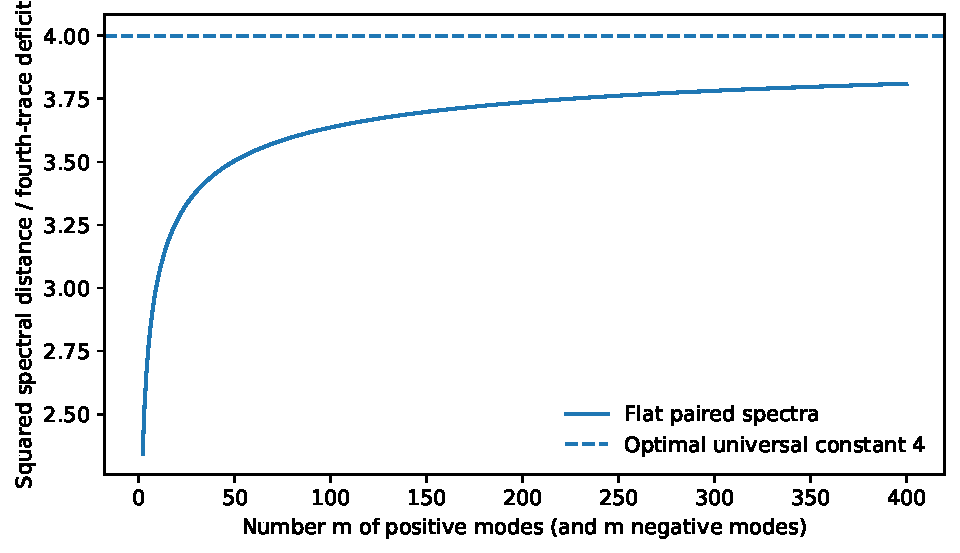
\includegraphics[width=.77\textwidth]{figures/rigidity_constant.pdf}
\caption{Flat paired spectra show that the constant $4$ in $D^2\leq4\Delta_4$ at zero skewness cannot be improved uniformly over dimensions. This sharpness sequence is distinct from the rank-two equality spectrum.}
\label{fig:rigidity}
\end{figure}

\subsection{The square-root distance exponent cannot improve}
For $0<r<1/2$, consider the four-coordinate spectrum
\begin{equation}\label{eq:sharp-exponent-spectrum}
\left(\sqrt{\frac{1-r}{2}},-\sqrt{\frac{1-r}{2}},
\sqrt{\frac r2},-\sqrt{\frac r2}\right).
\end{equation}
It has zero skewness and
\[
\gapfour=r(1-r),\qquad
D^2=2-2\sqrt{1-r}\sim r.
\]
Its fourth-moment deficit is exactly $48r(1-r)$. Hence spectral distance is of order the square root of the moment deficit. No uniform bound $D\leq C(36-\E Q^4)^\alpha$ can hold near the extremizer with $\alpha>1/2$.

\section{A sharp exponential-moment envelope and its tail consequences}
\label{sec:tails}

The test function $e^{tx}$ does not satisfy the polynomial-growth hypothesis, so it must not be inserted into \cref{thm:main} without justification. A direct application of the coefficient chord gives its own proof.

\begin{theorem}[Attained Laplace envelope]\label{thm:mgf}
For
\begin{equation}\label{eq:mgf-domain}
-\frac1{2b}<t<\frac1{2a},
\end{equation}
with a missing endpoint interpreted as infinite,
\begin{equation}\label{eq:mgf-envelope}
\E e^{tQ}\leq
\E e^{tY_\delta}
=\frac{e^{-(a-b)t}}{\sqrt{(1-2at)(1+2bt)}}.
\end{equation}
For $t\ne0$, equality holds precisely for the extremal spectrum.
\end{theorem}
\begin{proof}
Taylor's integral formula and \eqref{eq:R-representation} show that
\[
\frac{\psi(tz)}{z^2}
=2t^2\E\int_0^1(1-v)e^{tvzR}\dd v,
\]
with the continuous value used at $z=0$. This function is convex in $z$ on $[-b,a]$, and strictly convex if $t\ne0$. Integrability holds throughout \eqref{eq:mgf-domain}; compact subintervals of that domain justify the expectation. The logarithm of the left side in \eqref{eq:mgf-envelope} is
$\sum_i c_i^2\psi(tc_i)/c_i^2$. Apply \cref{lem:chord} and then \eqref{eq:psi}. Strictness follows from the strict chord, as in the moment proof.
\end{proof}

\subsection{Closed-form Chernoff optimization}
Let $\eta=a-b$, $d=ab$, and define
\begin{equation}\label{eq:K}
K_\delta(t)=-\eta t-\tfrac12\log(1-2\eta t-4dt^2).
\end{equation}
For $x\geq0$, Markov's inequality gives
\begin{equation}\label{eq:chernoff}
\Prob(Q\geq x)\leq e^{-I_\delta(x)},\qquad
I_\delta(x)=\sup_{0\leq t<1/(2a)}\{tx-K_\delta(t)\}.
\end{equation}
For $|\delta|<1$ and $x>0$, the unique optimizer is
\begin{equation}\label{eq:tstar}
t_*(\delta,x)=
\frac{x}{1+\eta x+\sqrt{(1+\eta x)^2+4dx(x+\eta)}}.
\end{equation}
The expression under the square root can also be written
\begin{equation}\label{eq:disc}
(1+2d)(x+\eta)^2+4d^2,
\end{equation}
which is nonnegative without cancellation. To verify \eqref{eq:tstar}, differentiate \eqref{eq:K}. The stationarity equation is
\begin{equation}\label{eq:saddle}
4d(x+\eta)t^2+2(1+\eta x)t-x=0.
\end{equation}
Strict convexity of $K_\delta$ and $K_\delta'(0)=0$ identify the positive solution within the moment-generating-function domain. The formula remains valid when $x+\eta=0$ by its rationalized form.

For numerical work, if $1+\eta x<0$, use the equivalent expression
\begin{equation}\label{eq:stable-root}
t_*=
\frac{\sqrt{(1+2d)(x+\eta)^2+4d^2}-(1+\eta x)}{4d(x+\eta)}
\end{equation}
to avoid subtractive cancellation in the denominator of \eqref{eq:tstar}. This issue is relevant when $\delta$ is close to $-1$.

At $\delta=1$, $t_*=x/[2(1+x)]$. At $\delta=-1$, $Q=1-g^2$: for $0\leq x<1$, $t_*=x/[2(1-x)]$, while for $x\geq1$ the upper-tail probability is zero and the limiting Chernoff rate is infinite. At $x=0$ all formulas are interpreted as $t_*=I_\delta(0)=0$.

\subsection{Zero-skewness formula and the optimal exponential scale}
At $\delta=0$, let $r_x=\sqrt{1+2x^2}$. Then
\begin{equation}\label{eq:zero-tail}
\Prob(Q\geq x)
\leq\sqrt{\frac{1+r_x}{2}}
\exp\!\left(-\frac{r_x-1}{2}\right),\qquad x\geq0.
\end{equation}
The same bound applies to $\Prob(Q\leq-x)$, although $Q$ itself need not be symmetric. A two-sided bound is twice the displayed expression, capped at one.

\begin{figure}[htbp]
\centering
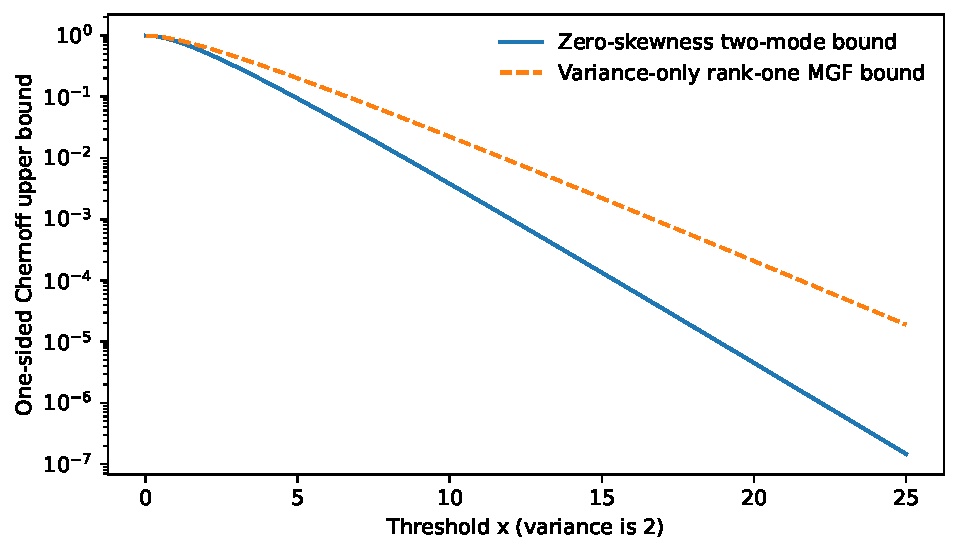
\includegraphics[width=.79\textwidth]{figures/tail_bounds.pdf}
\caption{Right-tail Chernoff bounds under variance $2$. Zero skewness permits a strictly improved spectral endpoint and exponential scale. The variance-only reference is obtained from the rank-one positive Laplace envelope; the curves are upper bounds, not actual tail probabilities.}
\label{fig:tails}
\end{figure}

\begin{proposition}[Sharp exponential scale, not a sharp prefactor]\label{prop:tail-scale}
Fix $|\delta|<1$. As $x\to\infty$,
\begin{equation}\label{eq:tail-asymptotic}
\Prob(Y_\delta>x)
\sim a\sqrt{\frac{2}{\pi(a+b)}}\,
 e^{-(a-b)/(2a)}x^{-1/2}e^{-x/(2a)}.
\end{equation}
Consequently, no right-tail estimate uniform over the fixed-$\delta$ class can have exponential coefficient greater than $1/(2a)$ with a subexponential prefactor. At zero skewness this coefficient is $1/\sqrt2$, compared with $1/2$ when only the variance is known.
\end{proposition}
\begin{proof}
Condition on $h$. Since $Y_\delta=ag^2-bh^2-(a-b)$,
\[
\Prob(Y_\delta>x)=
\E\Prob\!\left(g^2>\frac{x+a-b+bh^2}{a}\,\middle|\,h\right).
\]
The elementary Gaussian tail asymptotic gives
$\Prob(g^2>z)\sim\sqrt{2/\pi}\,z^{-1/2}e^{-z/2}$.
For all sufficiently large $x$, the usual upper Gaussian tail bound supplies an integrable dominating function after multiplying by $x^{1/2}e^{x/(2a)}$: it is a constant times $e^{-bh^2/(2a)}$. Dominated convergence yields
\[
\sqrt{\frac{2a}{\pi}}\,e^{-(a-b)/(2a)}
\E e^{-bh^2/(2a)}
=a\sqrt{\frac{2}{\pi(a+b)}}\,e^{-(a-b)/(2a)}.
\]
The law $Y_\delta$ belongs to the admissible class, so it obstructs every larger exponential coefficient. At zero skewness $a=1/\sqrt2$. For the matching universal upper scale, note that $\sum_i c_i^r\leq\sum_i|c_i|^r\leq1$ for every integer $r\geq2$. The positive-coefficient series in \eqref{eq:psi} therefore gives $\log\E e^{tQ}\leq\psi(t)$ for $0\leq t<1/2$. Its optimized bound has exponential scale $1/2$, and the admissible rank-one law $g^2-1$ prevents any improvement without additional information.
\end{proof}

The Chernoff upper bound generally has a different polynomial prefactor from \eqref{eq:tail-asymptotic}. We claim the exact Laplace supremum and the optimal exponential scale, not exact minimax tail probabilities.

\section{What the comparison does not imply}
\label{sec:notstoch}

The class $\fourth$ contains $f_t(z)=(z-t)_+^3$, because $f_t''(z)=6(z-t)_+$ is convex. Therefore
\begin{equation}\label{eq:stoploss}
\E(Q-t)_+^3\leq\E(Y_\delta-t)_+^3.
\end{equation}
For $t<x$, this implies the valid tail bound
\begin{equation}\label{eq:stoploss-tail}
\Prob(Q\geq x)\leq
\inf_{t<x}\frac{\E(Y_\delta-t)_+^3}{(x-t)^3}.
\end{equation}
It does \emph{not} imply $\Prob(Q>x)\leq\Prob(Y_\delta>x)$ pointwise.

Here is a concrete obstruction. Take the spectrum $(1/2,1/2,-1/2,-1/2)$. The resulting $Q$ is the difference of two independent exponential variables of mean one, hence has the centered Laplace law with density $e^{-|x|}/2$. It has variance $2$ and zero skewness. The comparator $Y_0=\sqrt2 UV$ has much more mass very close to zero: for small $x>0$,
\[
\Prob(|Y_0|\leq x)\geq c\,x\log(1/x)
\]
for an absolute $c>0$. To see this, integrate over $x\leq |U|\leq1$ and use that the Gaussian density of $V$ is bounded below near zero. By contrast, $\Prob(|Q|\leq x)=1-e^{-x}\sim x$. Both laws are symmetric and continuous, so for all sufficiently small positive $x$,
\[
\Prob(Q>x)>\Prob(Y_0>x).
\]
Thus the tail interpretation must pass through \eqref{eq:chernoff} or \eqref{eq:stoploss-tail}; replacing the random variable inside a tail indicator would be incorrect.

\section{Extensions beyond a single Gaussian square}
\label{sec:extensions}

\subsection{Common-shape centered Gamma inputs}
\begin{theorem}[Gamma extension]\label{thm:gamma}
Let $\alpha>0$, and let $Z_i$ be independent copies of
$\GammaDist(\alpha,1)-\alpha$. For $\sum_i c_i^2=1$ and $\delta=\sum_i c_i^3$,
\begin{equation}\label{eq:gamma-order}
\sum_i c_iZ_i\preceq_4 aZ_1'-bZ_2',
\end{equation}
where the primed variables are independent copies and $a,b$ are given by \eqref{eq:ab}. For $p\geq3$, equality in the resulting absolute-moment bound holds exactly for the same two-endpoint spectra.
\end{theorem}
\begin{proof}
The centered Gamma cumulant exponent has L\'evy measure
$\alpha e^{-r}\dd r/r$ on $(0,\infty)$. Repeat \cref{sec:proof} with this common base measure. The coefficient enclosure and chord are unchanged; the second-order Taylor remainder produces the same squared weights. Uniform exponential moments follow at a sufficiently small fixed $|t|$. Strictness for $p>3$ follows from the strict chord. For $p=3$, the interpolation contains a difference of two independent positive-shape Gamma variables whenever $a,b>0$ and $0<u<1$, giving full support as before.
\end{proof}

The variance and third moment in \eqref{eq:gamma-order} are $\alpha$ and $2\alpha\delta$. The exact fourth-moment frontier is
\begin{equation}\label{eq:gamma-fourth}
\E\left(\sum_i c_iZ_i\right)^4
\leq3\alpha^2+6\alpha T_\delta.
\end{equation}
At zero skewness, the extremizer is $(A-B)/\sqrt2$ with $A,B$ independent $\GammaDist(\alpha,1)$. Its characteristic function is $(1+t^2/2)^{-\alpha}$, so it equals in distribution $\sqrt W\,N$, where $W\sim\GammaDist(\alpha,1)$ and $N\sim N(0,1)$ are independent. Therefore the exact zero-skewness constant is
\begin{equation}\label{eq:gamma-zero}
\E\left|\frac{A-B}{\sqrt2}\right|^p
=\frac{2^{p/2}\Gamma(\alpha+p/2)\Gamma((p+1)/2)}{\Gamma(\alpha)\sqrt\pi}.
\end{equation}
Taking $\alpha=1/2$ and multiplying the centered inputs by $2$ recovers \eqref{eq:zero-moment}.

\subsection{A general infinitely divisible comparison}
\begin{proposition}\label{prop:ID}
Let $Z$ be a centered real infinitely divisible random variable with a finite exponential moment $\E e^{t_0|Z|}<\infty$ for some $t_0>0$. For independent copies $Z_i$, coefficients with $\sum_i c_i^2=1$, and $\delta=\sum_i c_i^3$,
\[
\sum_i c_iZ_i\preceq_4 aZ_1'-bZ_2'.
\]
Here $Z_1',Z_2'$ are independent copies of $Z$. No strict equality classification is asserted for this general base law.
\end{proposition}
\begin{proof}
Write the centered L\'evy exponent as a Gaussian part plus
$\int_{\R\setminus\{0\}}(e^{tr}-1-tr)\nu(\dd r)$.
The finite exponential moment and finite variance justify full linear compensation; near zero the compensated remainder is $O(r^2)$. The Gaussian part of the two weighted sums is the same, since their squared coefficient sums both equal one. Couple it as an independent common Gaussian summand along the interpolation.

Truncate the remaining L\'evy measure to $|r|>\varepsilon$. The Poisson derivative and Taylor identity give, up to the nonnegative factor $r^2(1-v)$, the chord comparison for the function $z\mapsto f''(X+vzr)$. This function is convex also when $r<0$. Integrate \eqref{eq:chord} against $\nu(\dd r)$ and the interpolation parameter. Finite exponential moments at a smaller fixed argument give the same uniform-integrability passage to the untruncated limit as in \cref{sec:proof}.
\end{proof}

If $\kappa_3(Z)\ne0$, then $\delta=\kappa_3(\sum c_iZ_i)/\kappa_3(Z)$ and the constraint is observable through the third cumulant. If $\kappa_3(Z)=0$, all such sums have zero third cumulant; in that case $\delta$ is additional coefficient information, not recoverable from skewness. For a Gaussian base law every normalized weighted sum has the same distribution, illustrating why the equality theorem does not extend verbatim.

\subsection{Countably many Gaussian modes}
\begin{corollary}[Second-chaos extension]\label{cor:infinite}
Let $(c_i)_{i\geq1}\in\ell_2$ have squared norm one. The series
$Q=\sum_{i\geq1}c_i(g_i^2-1)$ converges in $L^2$, and with
$\delta=\sum_{i\geq1}c_i^3$ one has $Q\preceq_4Y_\delta$ and
$\E|Q|^p\leq F_p(\delta)$ for every $p\geq3$.
\end{corollary}
\begin{proof}
Independent centered summands have total variance $2$, giving $L^2$ convergence. Apply \cref{thm:main} to each nonzero partial coefficient vector after normalizing it to squared norm one. Its normalized cubic sum tends to $\delta$. The uniform bound \eqref{eq:psi-bound} gives exponential uniform integrability for all normalized partial sums. Since $a(\delta),b(\delta)$ are continuous, the comparison passes to the limit for polynomial-growth test functions.
\end{proof}

\section{Interpretation and applications}
\label{sec:applications}

\subsection{Quadratic fluctuations of a Gaussian field}
Suppose a Gaussian fluctuation field $X$ has mean zero and covariance $\Sigma\succeq0$. For a real symmetric observable matrix $M$, put
$B=\Sigma^{1/2}M\Sigma^{1/2}$. Then
\[
X^{\mathsf T}MX-\tr(M\Sigma)\eqd G^{\mathsf T}BG-\tr B.
\]
The theory applies whenever $B\ne0$, with
\[
s^2=\tr(B^2)=\tr((M\Sigma)^2),\qquad
\delta=\frac{\tr(B^3)}{\tr(B^2)^{3/2}}.
\]
The covariance may be singular. If $B=0$, the centered observable is identically zero and needs no normalization. For energy differences, $B$ is often indefinite, so retaining the third trace distinguishes a balanced fluctuation from a single dominant positive mode. No interacting-field or quantum distribution is assumed to be Gaussian merely because its first few moments are known.

\subsection{Gaussian stochastic trace estimation}
For independent $G_1,\ldots,G_N\sim N(0,I_n)$, define
\[
\widehat T_N=\frac1N\sum_{j=1}^NG_j^{\mathsf T}MG_j.
\]
Writing the estimator error as one quadratic form in $Nn$ coordinates shows that its coefficient scale is $s/\sqrt N$ and its normalized third trace is $\delta/\sqrt N$. Hence, for $p\geq3$,
\begin{equation}\label{eq:trace-estimator}
\E|\widehat T_N-\tr M|^p
\leq\left(\frac{s}{\sqrt N}\right)^pF_p(\delta/\sqrt N).
\end{equation}
The corresponding bound for the right tail is
\[
\Prob\!\left(\widehat T_N-\tr M\geq\frac{s}{\sqrt N}x\right)
\leq e^{-I_{\delta/\sqrt N}(x)}.
\]
These are universal bounds from only the second and third traces. They do not exploit the repeated-block spectrum completely. In particular, their standardized fourth-moment bound tends to $9$, not the Gaussian limit $3$ for a fixed matrix averaged many times. This is a deliberate information limitation, not a claim of asymptotic sharpness for repeated sampling. The exact fourth moment, when $\tr(M^4)$ is available, is better for that purpose.

\subsection{What computational improvement is supplied}
The work reduces an optimization over every dimension and spectrum, subject to two scalar constraints, to a single explicitly parameterized two-dimensional distribution. The tail optimizer requires only elementary arithmetic and a square root once $a,b$ are known. This is an exact reduction of the \emph{extremal bound evaluation} problem. It is not a new asymptotic running-time result for computing matrix traces, eigenvalues, or sampling a general spin system.

\section{Reproducible verification and audit boundaries}
\label{sec:verification}

The accompanying code is supplementary evidence and a reusable evaluation tool. It is not a substitute for the proofs. It contains no randomized proof claims and no assertions of machine-checked Lean formalization.

\subsection{Exact arithmetic}
The script \texttt{code/verify\_exact.py} uses Python integers, rational arithmetic, and SymPy polynomial identities. Its recorded run contains:
\begin{center}
\begin{tabular}{@{}lr@{}}
\toprule
Check category & Count\\
\midrule
Symbolic identities & 11\\
Coordinate-enclosure necessary inequalities & 97,054\\
Zero-skewness integer spectra examined & 77\\
Exact even-moment comparisons & 385\\
Exact rigidity sharpness-sequence checks & 149\\
\midrule
Total exact assertion checks & 97,599\\
\bottomrule
\end{tabular}
\end{center}
The coordinate tests examine the integer inequality
$(\sum_j c_j^3-c_i^3)^2\leq(\sum_jc_j^2-c_i^2)^3$ before normalization. The even moments are computed by an exact cumulant recurrence, not sampling. The finite input family is specified in the script; its role is to catch algebraic or normalization errors, not exhaust the real-valued theorem.

\subsection{Floating-point diagnostics}
The script \texttt{code/verify\_numeric.py}, with fixed seed $20261008$, checks 4,000 spectra in dimensions 2 through 64, plus 80 non-integer-order moment comparisons. The recorded run passed 76,100 numerical assertions, including enclosure, moments through order 12, moment stability, Laplace comparisons, spectral rigidity, and the Chernoff stationary equation. The largest reported combined fractional-moment quadrature diagnostic was less than $3.0\times10^{-9}$. Tiny negative gaps of order $10^{-14}$ are retained in the report rather than disguised as exact nonnegativity.

The fractional moments use the Fourier identity in \cref{app:fractional}, not Monte Carlo. The quoted diagnostic combines numerical quadrature estimates with a bound for a discarded characteristic-function tail; it is \emph{not} a certified floating-point interval. Selected rank-one and zero-skewness cases are independently cross-checked against one-dimensional integration and the closed Gamma formula.

The tests found a numerical cancellation issue in the direct rationalized saddle formula near $\delta=-1$. The code now switches between \eqref{eq:tstar} and \eqref{eq:stable-root}. Underflow of an extremely small Chernoff bound to zero is permitted in floating-point output; the finite logarithmic rate is also returned.

\subsection{Package and reproducibility}
The package includes the article source and PDF, bibliography, evaluation routines, exact and numerical tests, machine-readable results, plotting scripts, a claim-status ledger, and a formalization roadmap. The recorded environment uses Python 3.13.5, NumPy 2.3.5, and SciPy 1.17.0. The README gives build commands. Repository provenance is pinned in \texttt{provenance.json}; no external repository theorem is imported into the computations.

The strongest remaining audit needs are independent mathematical review of the comparison and equality proof, checking priority against a broader literature search, and formal verification of the finite coefficient geometry and interpolation limit argument. The calculations already performed do not establish any of these independently.

\section{Further research questions}
\label{sec:future}

\paragraph{1. The unconditioned interval $3\leq p<4$.}
The conditional problem is now reduced to the scalar function $F_p(\delta)$. Is
$F_p(\delta)\leq F_p(1)$ throughout this interval? A proof would settle the corresponding part of the unconditioned absolute-moment question. The fourth-convex comparison alone does not order $Y_\delta$ for different $\delta$, because their third moments differ. A useful next step is a derivative formula in $\eta$ for the two-dimensional integral \eqref{eq:F-integral} with a sign-controlled kernel.

\paragraph{2. What happens for $2<p<3$?}
Here $f''(x)=p(p-1)|x|^{p-2}$ is not convex, so the main proof stops for a genuine reason. Does the same rank-two spectrum still maximize the fixed-skewness problem, or can a higher-rank spectrum beat it? Numerical optimization should distinguish these alternatives before any attempted interpolation extension. A counterexample would precisely locate the boundary of the order-based method.

\paragraph{3. Best stability constants and the $p=3$ endpoint.}
The constant $4$ at zero skewness in \cref{thm:rigidity} is optimal, but the exact $K_\delta$ for $\delta\ne0$ is unknown here. Likewise, \cref{thm:moment-stability} does not optimize its coefficients. Determine the infimum of $(F_p(\delta)-\E|Q|^p)/\Delta_4$ and whether it stays positive at $p=3$ for fixed interior $\delta$. The strictness proof at $p=3$ suggests studying the interpolation's probability of crossing the kink of absolute value.

\paragraph{4. Exact worst-case tail probabilities.}
Find $\sup\Prob(Q\geq x)$ at fixed $\delta$. The counterexample in \cref{sec:notstoch} rules out a universal answer obtained simply by inserting $Y_\delta$. The cubic stop-loss envelope may yield a more informative dual formulation, but attainment of the Laplace envelope is not enough to prove attainment of its optimized Markov bound.

\paragraph{5. Noncentral and mixed-degree Gaussian observables.}
For $G^{\mathsf T}MG+\ell^{\mathsf T}G-\tr M$, the cumulants involve both the spectrum and the alignment of $\ell$ with its eigenspaces. Can a bounded number of modes still attain the extremum when variance and skewness are fixed? The coefficient enclosure in \cref{lem:enclosure} must be replaced rather than assumed unchanged.

\paragraph{6. Additional information and effective rank.}
The trace-estimation discussion shows that two trace constraints cannot encode a repeated-block or high-effective-rank structure. Determine the exact extremizer after also bounding $\max_i|c_i|$ or fixing $\sum_i c_i^4$. A finite-support moment problem for the squared-coefficient measure is a plausible starting point, but its atom weights must remain compatible with actual coefficient multiplicities.

\paragraph{7. Certified evaluation and formalization.}
Develop interval-certified evaluation of $F_p(\delta)$ for fractional $p$, including uniform error bounds near $p=3$ and $|\delta|=1$. A formalization can begin with the enclosure and the exact fourth-trace identity, then prove the finite compound-Poisson derivative and the uniform-integrability limit. The full theorem should not be represented as certified merely by formalizing its final scalar inequality under the comparison as an axiom.

\appendix
\section{Moment recurrence and exact arithmetic}
\label{app:moments}

Let $m_k=\E Q^k$ and $m_0=1$. Differentiating the identity between the moment-generating function and the exponential of its cumulant series gives
\begin{equation}\label{eq:recurrence}
m_n=\sum_{r=1}^n\binom{n-1}{r-1}\kappa_r m_{n-r}
=\sum_{r=2}^n\binom{n-1}{r-1}
2^{r-1}(r-1)!\left(\sum_i c_i^r\right)m_{n-r}.
\end{equation}
For unnormalized integer or rational coefficients, every quantity is exact in integer or rational arithmetic. A normalized even moment is obtained afterward by division by $(\sum_i c_i^2)^{n/2}$ when $n$ is even, avoiding algebraic square roots. This is the method used by the exact tests.

The coefficient-defect identity itself is a polynomial identity subject only to $a^2+b^2=1$ and the specified second and third sums. It can be checked symbolically independently of every probability argument. By contrast, checking moments through order 12 cannot establish the comparison for all real $p$ or all test functions.

\section{A numerical formula for fractional absolute moments}
\label{app:fractional}

For $2<p<4$ and a centered real $X$ with finite $p$th moment,
\begin{equation}\label{eq:fractional}
\E|X|^p
=-\frac{2\Gamma(p+1)\sin(\pi p/2)}{\pi}
\int_0^\infty
\frac{\Re\varphi_X(t)-1+\tfrac12t^2\E X^2}{t^{p+1}}\dd t.
\end{equation}
One obtains the scalar identity by substituting $u=t|x|$ and integrating the compensated cosine kernel by parts; the coefficient is positive on $(2,4)$. The integrand before expectation is nonnegative because $\cos u\geq1-u^2/2$, so Tonelli's theorem justifies the expectation identity.

For the normalized quadratic form,
\begin{equation}\label{eq:charfun}
\varphi_Q(t)=\exp\left\{\sum_i\left[-itc_i-\tfrac12\log(1-2itc_i)\right]\right\}.
\end{equation}
The numerical routine subtracts the first two even terms analytically and evaluates a high-order moment expansion near zero to avoid catastrophic cancellation. For the tail, it integrates the polynomial compensation explicitly and only truncates the characteristic-function part. Since $|\varphi_Q(t)|\leq1$, the discarded part beyond $T$ has absolute value at most
\[
\frac{2\Gamma(p+1)|\sin(\pi p/2)|}{\pi p}\,T^{-p}.
\]
Floating-point evaluation of the integrand and the local Taylor truncation still require certification for an interval-proof claim; the present script labels its errors as diagnostics accordingly.

\clearpage
\bibliographystyle{plain}
\bibliography{references}
\end{document}
